\documentclass{article}
\usepackage{listings}
\usepackage{amsmath}
\usepackage{tikz}
\usepackage{color} %red, green, blue, yellow, cyan, magenta, black, white

\begin{document}

\definecolor{mygreen}{RGB}{28,172,0} % color values Red, Green, Blue
\definecolor{mylilas}{RGB}{170,55,241}

\lstset{language=Matlab,%
    basicstyle=\footnotesize\ttfamily,
    breaklines=false,%
    morekeywords={matlab2tikz},
    keywordstyle=\color{blue},%
    morekeywords=[2]{1}, keywordstyle=[2]{\color{black}},
    identifierstyle=\color{black},%
    stringstyle=\color{mylilas},
    commentstyle=\color{mygreen},%
    showstringspaces=false,%without this there will be a symbol in the places where there is a space
    emph=[1]{for,end,break},emphstyle=[1]\color{red}, %some words to emphasise
    %emph=[2]{word1,word2}, emphstyle=[2]{style},
}

\begin{centering}
	{\scshape\Large FMA240 - Handin 2\par}
	\vspace{0.5cm}
	Kristoffer Lundgren \texttt{<kem01klu@student.lu.se>}\par
	Stefan Eng \texttt{<atn08sen@student.lu.se>}\par
    \vspace{0.5cm}
	\today\par
    \rule{\textwidth}{0.4pt}
\end{centering}

\section*{Exercise 1}
  \noindent
  \textit{Construction of boundy.m and branchy.m functions.}

  \subsection*{boundy.m}

  \begin{lstlisting}
function bounds=boundy(x,D,minmax);
% function bounds=boundy(x,D,minmax);
% calculates the 1x2 vector with lower and upper bound
% respectively,
% given the 1xn vector with the current path,
% the NxN distance matrix D and the Nx2 matrix
% minmax, where minmax(i,1) is the minimum distance
% from city i and minmax(i,2) is the maximum distance
% from city i.

    % Get the number of cities.
    [~, N] = size(D);

    % Enumerate cities, unset cities already in path.
    remaining_cities = 1:N;
    remaining_cities(x) = [];

    % Calculate traveled distance and remaining min/max distances.
    sum_dim = 1; % Force the summation into a vector.
    remaining_minmax = sum(minmax(remaining_cities, :), sum_dim);
    current_distance = sum(diag(D(x(1:end-1), x(2:end))));

    bounds = remaining_minmax + current_distance;

    if (length(x) == N)
        % Visited all cities, add return length.
        bounds = bounds + D(x(end), x(1));
    else % Haven't reached the end, add minmax for last visit.
        bounds = bounds + minmax(x(end), :);
    end
end
  \end{lstlisting}

  \noindent
  The function takes the current path, the distance matrix, and an array that
  represents the minimum and maximum distance out from the cities.

  \newpage

  \subsection*{branchy.m}

  \begin{lstlisting}
function X=branchy(x,N);
% function X=branchy(x,N);
% returns the mx(n+1) matrix X where
% each row of X is a possible extension
% of the input path x.
% x is a 1xn vector, and N is the total number
% of cities in the problem.

     % Enumerate all cities 1 -> N, unset visited cities.
     remaining_cities = 1:N;
     remaining_cities(x) = [];

     % Set variables for row repetition.
     num_remaining = N-length(x);
     rep_col = 1; % Constrain repetition to one column.

     % Repeat current path num_remaining times, append remaining cities.
     X = [repmat(x, num_remaining, rep_col) remaining_cities'];
end
  \end{lstlisting}

  \noindent
  The function takes the current path and the total number of cities and
  returns a matrix where each row is a possible next step in the path. \\

\section*{Exercise 2}

  \textit{Run the travsalesman.m script with the supplied matrix D. The script
  will use the functions that were created in exercise 1, display the results.}

  \subsection*{Results from travsalesman.m}

  \begin{lstlisting}
>> [x, fopt] = travsalesman(D)

x =

     1     4     9     5     2     8     3     7     6


fopt =

    56
  \end{lstlisting}

  \noindent
  where x is the optimal path, and the total distance traveled is 56.

  \newpage

\section*{Exercise 3}

  \textit{Run the travsalesman.m script for traveling salesman problems of different
  sizes and plot the execution times as a function of the number of cities in
  the problem.}

  \subsection*{Results and plots}

  \begin{figure}[!h]
    \centering
    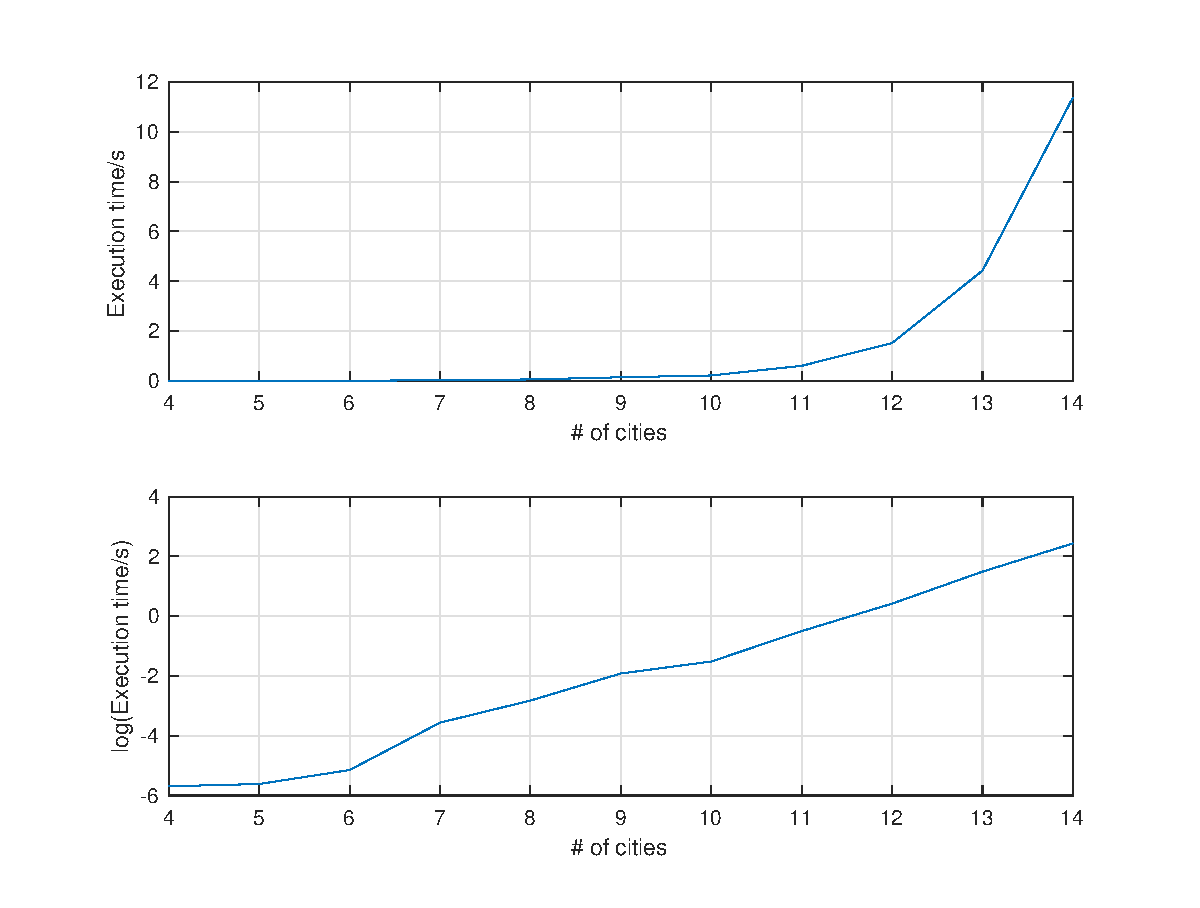
\includegraphics[width=0.9\textwidth]{4_14_20samples.eps}
  \end{figure}

  \noindent
  Result of running travsalesman.m for different travel-problems generated by
  \texttt{createdistancematrix.m} (attached), using the average of 20 samples for each city
  size between 4 and 14 cities and a maximum distance between any two cities of 200 units
  (a script automating this is attached as \texttt{runscript.m}). The semilog plot does indicate exponential behaviour (as it
  resembles a straight line)
  for solving the traveling salesman problem using the branch and bound algorithm.

\end{document}
